\chapter{Progettazione e implementazione del prototipo}
In seguito allo studio dell'algoritmo \textbf{\textit{wavefront}} si è passati a una fase di implementazione di un prototipo, che potesse andare a migliorare le prestazioni del tool \href{https://github.com/AlgoLab/RecGraph}{\textbf{\textit{RecGraph}}} \cite{Recgraph} nell'allineamento tra un \emph{grafo di variazione} e una \emph{sequenza}. In seguito vengono esposte la fasi di \textbf{progettazione} e \textbf{implementazione} del prototipo, per poi passare a un \textbf{benchmark} che va a confrontare le prestazioni dell'algoritmo \textbf{\textit{wavefront}} con quelle della implementazione di \textbf{\textit{RecGraph}}.   

\section{Progettazione}
    Nella seguente sezione vengono riportate le scelte prese in \textbf{fase di progettazione} del prototipo e la \textbf{struttura architetturale} a cui hanno portato. L'intera implementazione del prototipo è disponibile al seguente link: \\
    \href{https://github.com/iFoxz17/WF_Recgraph}{https://github.com/iFoxz17/WF\_Recgraph.} 
\subsection{Organizzazione modulare}
    Si è scelto di organizzare il prototipo seguendo un approccio ad \emph{elevata modularità}, in maniera da rendere più semplice l'integrazione di eventuali future modifiche o migliorie:
    
    \begin{figure}[ht]
        \centering
        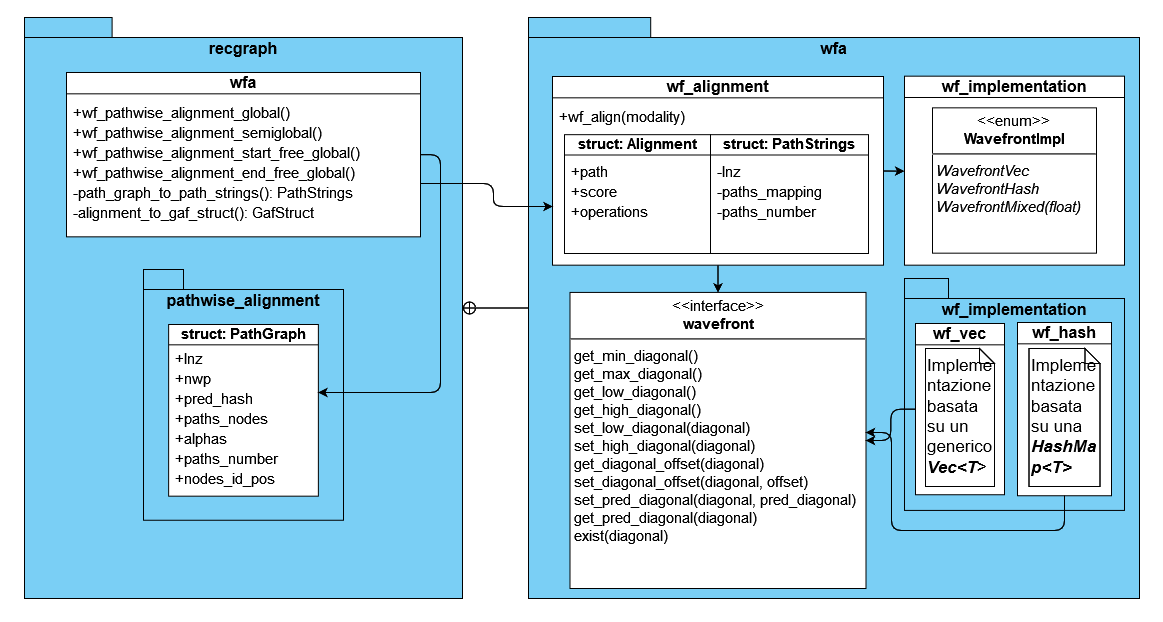
\includegraphics[width=1\linewidth]{images/wf_modules.png}
        \caption[Organizzazione modulare del prototipo]{\emph{Organizzazione modulare} del prototipo.}
        \label{fig:wf_modules}
    \end{figure}

    Come è possibile vedere dalla figura \ref{fig:wf_modules}, viene definita un'interfaccia \textbf{\textit{wfa}} che espone le quattro modalità di allineamento implementate:
    \begin{itemize}
        \item \textbf{\textit{wf\_pathwise\_alignment\_global}}, performa un allineamento in \emph{modalità globale};
        \item \textbf{\textit{wf\_pathwise\_alignment\_semiglobal}}, performa un allineamento in \emph{modalità semiglobale};
        \item \textbf{\textit{wf\_pathwise\_alignment\_start\_free\_global}}, performa un allineamento che può iniziare da qualsiasi vertice del grafo, ma vincolato a finire necessariamente nell'ultimo nodo;
        \item \textbf{\textit{wf\_pathwise\_alignment\_end\_free\_global}}, performa un allineamento che può finire in qualsiasi vertice del grafo, ma vincolato a iniziare necessariamente nel primo nodo.
    \end{itemize}
    Inoltre, all'interno del modulo sono contenute altre funzioni per convertire le \emph{strutture dati} utilizzate da \textbf{\textit{RecGraph}} in quelle utilizzate all'interno del package \textbf{\textit{wfa}}, contenente le seguenti componenti:
    \begin{itemize}
        \item \textbf{\textit{wavefront}}: interfaccia per definire le operazioni che deve implementare una struttura volta a rappresentare un \emph{fronte d'onda};
        \item \textbf{\textit{wf\_implementation}}: modulo che contiene le implementazioni disponibili per rappresentare un \emph{fronte d'onda} (devono implementare l'interfaccia \textbf{\textit{wavefront}});
        \item \textbf{\textit{wf\_alignment}}: modulo contenente le funzioni e le strutture dati che effettuano l'allineamento utilizzando l'algoritmo \textbf{\textit{wavefront}}.
    \end{itemize}
\subsection{Integrazione in RecGraph}
    Per integrare il protopipo all'interno di \textbf{\textit{RecGraph}} (al fine di utilizzare le già implementate funzionalità di lettura e scrittura di grafi) si è utilizzato il modulo \textbf{\textit{wfa}}, utilizzando direttamente le funzioni di allineamento esposte al posto di quelle di \textbf{\textit{RecGraph}}; lo stesso modulo si occupa della conversione delle differenti strutture dati utilizzate. La figura \ref{fig:wf_integration} mostra la \emph{struttura modulare} di \textbf{\textit{RecGraph}} e come è stato integrato il prototipo al suo interno.
        
    \begin{figure}[H]
        \centering
        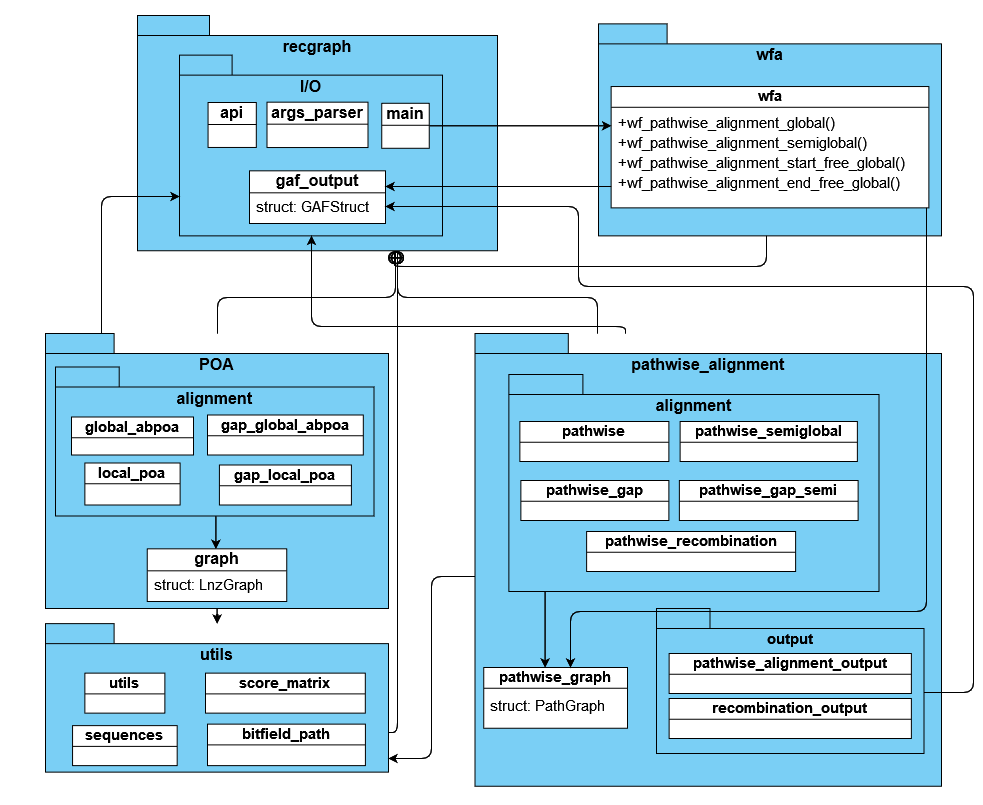
\includegraphics[width=1\linewidth]{images/wf_integration.png} 
        \caption[Integrazione]{Integrazione del prototipo in \textbf{\textit{RecGraph}}.}
        \label{fig:wf_integration}
    \end{figure}
    \vspace{20pt}
    \noindent
    Come è possibile vedere dalle \emph{relazioni di dipendenza}, il prototipo si serve soltanto delle due strutture dati \textbf{\textit{pathwise\_graph}} e \textbf{\textit{gaf\_output}}, utilizzate rispettivamente per rappresentare un \emph{grafo di variazione} e per contenere le informazioni di un allineamento in formato \emph{gaf}; inoltre, esso viene utilizzato direttamente all'interno del \textbf{\textit{main}}. Si riesce così a ottenere un basso accoppiamento dei moduli, pratica consigliata da \emph{design pattern} come \emph{low coupling}, al fine di diminuire l'impatto di eventuali futuri cambiamenti sul sistema.  

\section{Implementazione}
    In questa sezione si discutono le \textbf{scelte implementative} prese nella costruzione del prototipo, sviluppato tramite il linguaggio di programmazione \href{https://www.rust-lang.org/it}{\textbf{\textit{Rust}}.} 

\subsection{Interfaccia \textit{wavefront}}
    Modulo che definisce il \emph{trait} \textbf{\textit{Wavefront}} (struttura utilizzata in \textbf{\textit{Rust}} per definire un'\emph{interfaccia}), il quale specifica le operazioni che devono essere implementate per rappresentare un \emph{fronte d'onda}; per mantenere la complessità in tempo dell'algoritmo \emph{wavefront}, tutte le operazioni devono eseguite in $O(1)$. 
    
\subsection{Modulo \textit{wf\_implementation}}
    Modulo che definisce le implementazioni disponibili per rappresentare un \emph{fronte d'onda}: le definizioni si trova all'interno della \emph{enum} \textbf{\textit{WavefrontImpl}}, mentre le effettive implementazioni nel \emph{sotto-package} \textbf{\textit{wf\_implementation}} (figura \ref{fig:wf_modules}). In particolare, sono state fornite due implementazioni:
    \begin{itemize}
        \item \textbf{\textit{wf\_vec}}, memorizza il valore degli offsets delle diagonali all'interno di un \textbf{\textit{Vec}}; risulta \emph{più veloce} dell'altra implementazione, ma necessità di salvare anche gli offset delle diagonali che non vengono computate, generando uno \emph{spreco di memoria} e portando la \textbf{complessità in spazio} a 
        \begin{equation}
            T(n, m, p, \overline{d}) = O((n+m) \cdot \overline{d} \cdot p)
            \label{equation:space_complexity_wf_vec}
        \end{equation}
        \item \textbf{\textit{wf\_hash}}, salva il valore degli offsets delle diagonali all'interno di una \textbf{\textit{HashMap}}; può risultare particolarmente \emph{efficiente in memoria} quando il numero delle diagonali effettivamente computate è molto inferiore al totale, permettendo di evitare la memorizzazione di tutte le diagonali che non vengono computate e mantenendo l'\emph{andamento in memoria} a 
        \begin{equation}
            T(n, m, p, \overline{d}) = O(\overline{d}^2 \cdot p)
            \label{equation:space_complexity_wf_hash}
        \end{equation}
    \end{itemize}
    E' stata definita anche una terza implementazione, \textbf{\textit{WavefrontMixed}}, che cerca di unire i \emph{punti di forza} delle altre due: finchè la \emph{percentuale delle diagonali} che si sta computando è minore a una certa \textit{soglia parametrizzata}, viene scelto l'approccio \textbf{\textit{WavefrontHash}}, risparmiando così \emph{memoria} senza perdere troppo in \emph{tempo} (scegliendo soglie abbastanza basse, le diagonali effettivamente computate risultano molto inferiori a quelle totali, e la maggior parte del tempo dell'allineamento è richiesto quando il numero di diagonali che si stanno trattando cresce); superata la soglia, si passa invece all'implementazione \textbf{\textit{WavefrontVec}}, di cui viene ridotto lo \emph{spreco di memoria} (siccome il numero di diagonali che si stanno computando è vicino al massimo) e che risulta \emph{più veloce}.  
    
    Inoltre, il \emph{tipo degli interi} con cui vengono salvati gli offset risulta \emph{generico} sia in \textbf{\textit{wf\_vec}} che in \textbf{\textit{wf\_hash}}: a seconda delle dimensioni del \emph{grafo} e delle \emph{reads} in ingresso viene scelto in automatico il tipo più piccolo tra quelli disponibili (\textbf{\textit{u8}}, \textbf{\textit{u16}}, \textbf{\textit{u32}}, \textbf{\textit{u64}} e \textbf{\textit{u128}}), permettendo un significativo \emph{risparmio di memoria} (si osservi che per grafi con fino a 65535 nodi è possibile utilizzare degli \textbf{\textit{u16}}). 

\subsection{Modulo \textit{wf\_alignment}}
\label{section:wf_alignment}
    Modulo che si occupa di effettuare effettivamente l'allineamento tra il \emph{grafo di variazione} e la \emph{sequenza}. Nella figura \ref{fig:wf_alignment} viene fornito un diagramma che illustra le sue componenti più importanti:
    \begin{figure}[h]
        \centering
        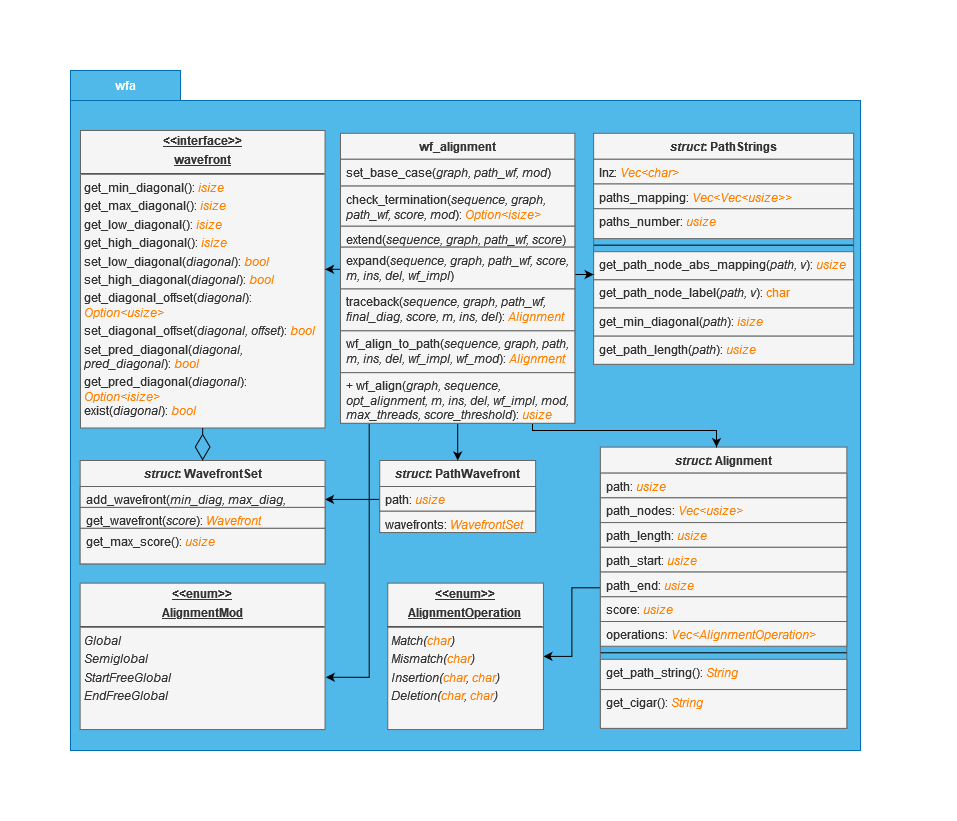
\includegraphics[width=1\linewidth]{images/wf_alignment_diagram.png} 
        \caption[Modulo allineamento]{Modulo \emph{wf\_alignment} per la gestione dell'allineamento.}
        \label{fig:wf_alignment}
        \end{figure}
    \clearpage

    In ingresso, il \emph{grafo di variazione} viene memorizzato tramite la \textbf{\textit{struct PathStrings}}, che essenzialmente estrae tutti i cammini del grafo; in output, invece, viene restituita un'istanza della \textbf{\textit{struct Alignment}}, contenente tutte le informazioni dell'allineamento effettuato.
    L'insieme dei \emph{fronti d'onda} computati per ogni \emph{punteggio} viene memorizzato nella \textbf{\textit{struct WavefrontSet}}: questa, insieme al \emph{cammino} che si sta trattando, va a comporre la \textbf{\textit{struct PathWavefront}}, che contiene tutte le informazioni necessarie per effettuare l'allineamento a un percorso.
    A livello di interfaccia viene esposta solamente una funzione, \textbf{\textit{wf\_align}}, che si occupa di gestire gli allineamenti tra i percorsi del grafo, lanciando un \emph{thread} per ogni percorso e selezionando il miglior allineamento trovato. In particolare, riceve in ingresso\footnote{Per ragioni di leggibilità, sono stati riportati solo i parametri più importanti.}
    \begin{itemize}
        \item \emph{il grafo di variazione} (come \textbf{\textit{PathStrings}}),
        \item la \emph{sequenza} da allineare,
        \item un \emph{array} dove inserire gli allineamenti ottimali trovati (come \textbf{\textit{Alignment}}),
        \item le \emph{penalità} di \textbf{\textit{mismatch}}, \textbf{\textit{inserimento}} e \textbf{\textit{cancellazione}}.
        \item la \emph{modalità di allineamento} (una voce della \emph{enum} \textbf{\textit{AlignmentMod}}),
        \item il numero massimo di \emph{thread} da eseguire in parallelo,
        \item una \emph{soglia} a cui troncare l'allineamento (facoltativa)
    \end{itemize}
    e restituisce il valore dell'allineamento prodotto. Inoltre, ogni volta che un thread termina un allineamento, viene impostata (o eventualmente aggiornata) una \emph{soglia} sul \emph{massimo punteggio raggiungibile}, condivisa da tutti i thread: ogni allineamento che supera tale soglia viene abbandonato. 
    Ogni thread lanciato esegue la funzione \textbf{\textit{wf\_align\_to\_path}}, che esegue l'algoritmo \emph{wavefront} tra un percorso del grafo e una sequenza (quindi tra due stringhe), alternando le già discusse fasi di \emph{estensione} ed \emph{espansione}.
\clearpage

\section{Benchmark}
    In seguito vengono riportate alcune sperimentazioni eseguite per osservare il comportamento del prototipo. In particolare, nella prima sezione si analizzano le performance dell'\emph{allineamento} \textbf{\textit{wavefront}} rispetto a \textbf{\textit{RecGraph}}, mentre nella sezione successiva si tratta l'andamento delle prestazioni del prototipo rispetto a diversi \textbf{gradi di libertà} (\emph{punteggio dell'allineamento}, \emph{numero di thread utilizzati}, \emph{numero di cammini del grafo di variazione}). La sperimentazione è stata eseguita su un server con 64 core e 256 GB di RAM. Per quanto riguarda le grandezze in input, si fa riferimento alla seguente notazione:
    \begin{itemize}
        \item \textbf{\textit{n}}: lunghezza media dei cammini del \emph{grafo di variazione};
        \item \textbf{\textit{p}}: numero di cammini del \emph{grafo di variazione};
        \item \textbf{\textit{m}}: lunghezza della \emph{sequenza};
        \item \textbf{\textit{d}}: valore ottimale dell'allineamento. 
    \end{itemize}

\subsection{RecGraph vs Wavefront}
\subsubsection{Grafo di variazione}
    In questa prima fase della sperimentazione è stato usato il \textbf{grafo di variazione} descritto nella tabella \ref{tab:graph}:
    \vspace{20pt}
    \begin{table}[ht]
        \centering
        \begin{tabular}{|c|c|c|c|}
        \hline
        \multicolumn{4}{|c|}{\multirow{2}{*}{\textbf{Variation graph}}} \\
        \multicolumn{4}{|c|}{} \\
        \hline
        \textbf{Linearization} & \multicolumn{3}{|c|}{\textbf{Paths}} \\
        \hline
        \textbf{Length (bp)} & \textbf{Number} & \textbf{Paths mean length (bp)} & \textbf{Paths for node} \\
        \hline
        49376 & 30 & 29744 & 18.1 (60\%) \\
        \hline
        \end{tabular}
        \caption{Caratteristiche del \emph{grafo di variazione} usato nel benchmark.}
        \label{tab:graph}
    \end{table}
    \vspace{10pt}
    
    In questa istanza si nota un'importante \emph{sovrapposizione dei cammini}: per ogni nodo, infatti, passano in media 18 cammini su 30 totali (più del 60\%). Questa caratteristica va a penalizzare l'implementazione dell'algoritmo \textbf{\textit{wavefront}} in quanto, basandosi sull'estrazione dei cammini dal grafo per permettere il \textbf{\textit{multithreading}}, va a computare diverse volte i valori degli allineamenti per gli stessi nodi condivisi da più percorsi; al contrario, \textbf{\textit{RecGraph}} sfrutta a suo vantaggio questa proprietà, memorizzando soltanto il punteggio di un solo percorso per i nodi condivisi (ottimizzazione del \textbf{\textit{reference path}} (sezione \ref{section:recgraph})).   

    \vspace{20pt}
    Si riportano i risultati ottenuti su \textbf{reads} di diversa lunghezza, sia in \textbf{modalità globale} che in \textbf{modalità semiglobale}.

\subsubsection{Modalità globale}
    Per la sperimentazione in \textbf{modalità globale} sono state usate \emph{sequenze} di lunghezza 150 bp, 1000 bp, 10000 bp e 25000 bp; i seguenti valori rigurdano allineamenti eseguiti utilizzando \textbf{\textit{RecGraph}}:
    \vspace{20pt}
    \begin{table}[h]
        \centering
        \begin{tabular}{|c|c|c|c|c|c|c|c|}
        \hline
        \multicolumn{8}{|c|}{\multirow{2}{*}{\textbf{Modality:} \emph{Global}}} \\
        \multicolumn{8}{|c|}{} \\
        \hline
        & \multicolumn{2}{|c|}{\textbf{Reads}} & \multicolumn{4}{|c|}{\textbf{Time (s)}} & \textbf{Memory (GB)} \\
        \hline
        \textbf{Algorithm} & \textbf{N} & \textbf{L} & \textbf{Tot} & \textbf{Mean} & \textbf{Max} & \textbf{Min} & \textbf{Max} \\
        \hline
        \multirow{4}{*}{\emph{RecGraph}} & 25 & 150 & 75 & 3.0 & 3.6 & 2.5 & 2.17 \\
        \cline{2-8}
        & \multirow{2}{*}{10} & 1000 & \multirow{2}{*}{214} & 21.4 & 26.4 & 20.0 & 7.84 \\
        & & $6.7 \times$ & & $7.1 \times$ & $7.3 \times$ & $8 \times$ & $3.6 \times$ \\
        \cline{2-8}
        & \multirow{2}{*}{5} & 10000 & \multirow{2}{*}{1155} & 231.1 & 241.4 & 216.2 & 75.64 \\
        & & $66.7 \times$ & & $77.0 \times$ & $67.1 \times$ & $86.5 \times$ & $34.8 \times$ \\
        \cline{2-8}
        & \multirow{2}{*}{5} & 25000 & \multirow{2}{*}{6909} & 690.9 & 703.2 & 678.5 & 192.45 \\
        & & $167 \times$ & & $230 \times$ & $195 \times$ & $271.4 \times$ & $88.7 \times$ \\
        \hline
        \end{tabular}
        \caption{Benchmark per \textbf{\textit{RecGraph}} in \emph{modalità globale}.}
        \label{tab:benchmark_RecGraph_global}
    \end{table}
    \vspace{10pt}
    
   I dati evidenziano una \textbf{complessità lineare} nella \textit{lunghezza delle sequenze}, sia per quanto riguarda il \textbf{tempo} che per lo \textbf{spazio}, in linea con la complessità $O(n \cdot m \cdot p)$ attesa. Sulle \textbf{reads} di lunghezza $25000$ bp inizia a essere necessaria anche un'importante quantità di memoria ($\approx$ 200 GB).
   
   \vspace{20pt} 
    A seguire invece i valori ottenuti dall'algoritmo \textbf{\textit{wavefront}} con \emph{distanza di edit unitaria}:
    \vspace{20pt}
    \begin{table}[h]
        \centering
        \begin{tabular}{|c|c|c|c|c|c|c|c|c|}
        \hline
        \multicolumn{9}{|c|}{\multirow{2}{*}{\textbf{Modality:} \emph{Global}}} \\
        \multicolumn{9}{|c|}{} \\
        \hline
        & \multicolumn{2}{|c|}{\textbf{Reads}} & \multicolumn{4}{|c|}{\textbf{Time (s)}} & \textbf{Memory (GB)} & \textbf{Score} \\
        \hline
        \textbf{Algorithm} & \textbf{N} & \textbf{L} & \textbf{Tot} & \textbf{Mean} & \textbf{Max} & \textbf{Min} & \textbf{Max} & \textbf{Mean} \\
        \hline
        \multirow{4}{*}{\emph{wf\_edit-distance}} & 25 & 150 & 545 & 21.8 & 24.5 & 20.2 & 111.33 & 28879 \\
        \cline{2-9}
        & \multirow{2}{*}{10} & 1000 & \multirow{2}{*}{222} & 22.2 & 24.9 & 20.2 & 110.32 & 28029 \\
        & & $6.7 \times$ & & $1.02 \times$ & $1.02 \times$ & $1 \times$ & $0.99 \times$ & $0.97 \times$\\
        \cline{2-9}
        & \multirow{2}{*}{5} & 10000 & \multirow{2}{*}{139.7} & 28.0 & 29.0 & 26.8 & 111.23 & 19669 \\
        & & $66.7 \times$ & & $1.28 \times$ & $1.18 \times$ & $1.34 \times$ & $1.0 \times$ & $0.68 \times$\\
        \cline{2-9}
        & \multirow{2}{*}{5} & 25000 & \multirow{2}{*}{134} & 13.4 & 15.1 & 12.1 & 64.42 & 8149\\
        & & $167 \times$ & & $0.6 \times$ & $0.6 \times$ & $0.6 \times$ & $0.58 \times$ & $0.28 \times$ \\
        \hline
        \end{tabular}
        \caption{Benchmark per \textbf{\textit{wf\_edit-distance}} in \emph{modalità globale}.}
        \label{tab:benchmark_wf_edit-dist_global}
    \end{table}
    \vspace{10pt}

    Qui si nota un andamento del tutto diverso: l'allineamento risulta \emph{meno performante} per le sequenze di lunghezza 150 bp, 1000 bp e 10000 bp (che producono punteggi di allineamento molto alti), mentre risulta più \emph{efficiente} per le sequenze di 25000 bp, migliorando sia in \textbf{tempo di esecuzione} sia in \textbf{memoria occupata} in accordo con la complessità $O(\min\{n, m\} \cdot \overline{d} \cdot p)$ prevista. 

    Di seguito un confronto dei valori ottenuti dalle esecuzioni di \textbf{\textit{RecGraph}} e di \textbf{\textit{wf\_edit-distance}} per sequenze della stessa lunghezza:

\vspace{20pt}
    \begin{table}[h]
        \centering
        \begin{tabular}{|c|c|c|c|c|c|}
            \hline
                \multicolumn{2}{|c|}{\textbf{Modality:} \emph{Global}} & \multicolumn{2}{|c|}{\textbf{Reads number: } \emph{25}} & \multicolumn{2}{|c|}{\textbf{Reads length:} \emph{150 bp}} \\
            \hline
                \multicolumn{6}{|c|}{} \\
            \hline
                & \multicolumn{4}{|c|}{\textbf{Time (s)}} & \textbf{Memory (GB)} \\
            \hline
                \textbf{Algorithm} & \textbf{Tot} & \textbf{Mean} & \textbf{Max} & \textbf{Min} & \textbf{Max} \\
            \hline
                \emph{RecGraph} & 75 & 3.0 & 3.6 & 2.5 & 2.17 \\
            \hline
                \multirow{2}{*}{\emph{wf\_edit-distance}} & 545 & 21.4 & 24.5 & 20.2 & 111.33 \\
                & $7.3 \times$ & $7.3 \times$ & $7.5 \times$ & $9 \times$ & $51 \times$ \\
            \hline
            \multirow{2}{*}{\emph{wf\_weighted\_edit-distance}} & 1097 & 43.9 & 47.1 & 43.0 & 223.59 \\
                & $14.6 \times$ & $14.6 \times$ & $13.1 \times$ & $17.2 \times$ & $103 \times$ \\
            \hline
        \end{tabular}
        \caption{Benchmark per \emph{reads} di 150 bp in \emph{modalità globale}. Nella modalità \textbf{\textit{wf\_weighted-edit-distance}}, sono state usate le seguenti penalità: \textbf{mismatch=1}, \textbf{insertion=2}, \textbf{deletion=2}.}
        \label{tab:benchmark_global_150}
    \end{table}
    \vspace{20pt}
    
    \begin{table}[h]
        \centering
        \begin{tabular}{|c|c|c|c|c|c|}
            \hline
                \multicolumn{2}{|c|}{\textbf{Modality:} \emph{Global}} & \multicolumn{2}{|c|}{\textbf{Reads number: }   \emph{10}} & \multicolumn{2}{|c|}{\textbf{Reads length:} \emph{1000 bp}} \\
            \hline
                \multicolumn{6}{|c|}{} \\
            \hline
                & \multicolumn{4}{|c|}{\textbf{Time (s)}} & \textbf{Memory (GB)} \\
            \hline
                \textbf{Algorithm} & \textbf{Tot} & \textbf{Mean} & \textbf{Max} & \textbf{Min} & \textbf{Max} \\
            \hline
                \emph{RecGraph} & 214 & 21.4 & 26.4 & 20.0 & 7.84 \\
            \hline
                \multirow{2}{*}{\emph{wf\_edit-distance}} & 222 & 22.2 & 24.9 & 20.2 & 110.32 \\
                & $1.04 \times$ & $1.04 \times$ & $0.94 \times$ & $1 \times$ & $14 \times$ \\
            \hline
            \multirow{2}{*}{\emph{wf\_weighted\_edit-distance}} & 464.0 & 46.4 & 46.9 & 46.0 & 223.61 \\
                & $2.2 \times$ & $2.2  \times$ & $1.78 \times$ & $2.3 \times$ & $28.5 \times$ \\
            \hline
        \end{tabular}
        \caption{Benchmark per \emph{reads} di 1000 bp in \emph{modalità globale}. Nella modalità \textbf{\textit{wf\_weighted-edit-distance}}, sono state usate le seguenti penalità: \textbf{mismatch=1}, \textbf{insertion=2}, \textbf{deletion=2}.}
        \label{tab:benchmark_global_1k}
    \end{table}
    \vspace{20pt}
    
    \begin{table}[h]
        \centering
        \begin{tabular}{|c|c|c|c|c|c|}
            \hline
                \multicolumn{2}{|c|}{\textbf{Modality:} \emph{Global}} & \multicolumn{2}{|c|}{\textbf{Reads number: } \emph{5}} & \multicolumn{2}{|c|}{\textbf{Reads length:} \emph{10000 bp}} \\
            \hline
                \multicolumn{6}{|c|}{} \\
            \hline
                & \multicolumn{4}{|c|}{\textbf{Time (s)}} & \textbf{Memory (GB)} \\
            \hline
                \textbf{Algorithm} & \textbf{Tot} & \textbf{Mean} & \textbf{Max} & \textbf{Min} & \textbf{Max} \\
            \hline
                \emph{RecGraph} & 1155 & 231.1 & 241.4 & 216.2 & 75.64 \\
            \hline
                \multirow{2}{*}{\emph{wf\_edit-distance}} & 139.7 & 28.0 & 29.0 & 26.8 & 111.23 \\
                & $0.12 \times$ & $0.12  \times$ & $0.12 \times$ & $0.12 \times$ & $1.47 \times$ \\
            \hline
            \multirow{2}{*}{\emph{wf\_weighted\_edit-distance}} & 287.0 & 57.3 & 56.4 & 59.6 & 196.73 \\
                & $0.25 \times$ & $0.25  \times$ & $0.23 \times$ & $0.28 \times$ & $2.6 \times$ \\
            \hline
        \end{tabular}
        \caption{Benchmark per \emph{reads} di 10000 bp in \emph{modalità globale}. Nella modalità \textbf{\textit{wf\_weighted-edit-distance}}, sono state usate le seguenti penalità: \textbf{mismatch=1}, \textbf{insertion=2}, \textbf{deletion=2}.}
        \label{tab:benchmark_global_10k}
    \end{table}
    \vspace{20pt}
\clearpage
    
    \begin{table}[h]
        \centering
        \begin{tabular}{|c|c|c|c|c|c|}
            \hline
                \multicolumn{2}{|c|}{\textbf{Modality:} \emph{Global}} & \multicolumn{2}{|c|}{\textbf{Reads number: } \emph{5}} & \multicolumn{2}{|c|}{\textbf{Reads length:} \emph{25000 bp}} \\
            \hline
                \multicolumn{6}{|c|}{} \\
            \hline
                & \multicolumn{4}{|c|}{\textbf{Time (s)}} & \textbf{Memory (GB)} \\
            \hline
                \textbf{Algorithm} & \textbf{Tot} & \textbf{Mean} & \textbf{Max} & \textbf{Min} & \textbf{Max} \\
            \hline
                \emph{RecGraph} & 6909 & 690.9 & 703.2 & 678.5 & 192.45 \\
            \hline
                \multirow{2}{*}{\emph{wf\_edit-distance}} & 134.0 & 13.4 & 15.1 & 12.1 & 64.42 \\
                & $0.02 \times$ & $0.02  \times$ & $0.02 \times$ & $0.02 \times$ & $0.33 \times$ \\
            \hline
                \multirow{2}{*}{\emph{wf\_weighted\_edit-distance}} & 190.0 & 19.0 & 20.9 & 17.7 & 95.16 \\
                & $0.03 \times$ & $0.03  \times$ & $0.03 \times$ & $0.03 \times$ & $0.49 \times$ \\
            \hline
        \end{tabular}
        \caption{Benchmark per \emph{reads} di 25000 bp in \emph{modalità globale}. Nella modalità \textbf{\textit{wf\_weighted-edit-distance}}, sono state usate le seguenti penalità: \textbf{mismatch=1}, \textbf{insertion=2}, \textbf{deletion=2}.}
        \label{tab:benchmark_global_25k}
    \end{table}
    \vspace{20pt}
    
    e una \textbf{visualizzazione grafica} dei dati precedentemente riportati (figura \ref{fig:global_comparison}):
    \begin{figure}[!h]
        \centering
        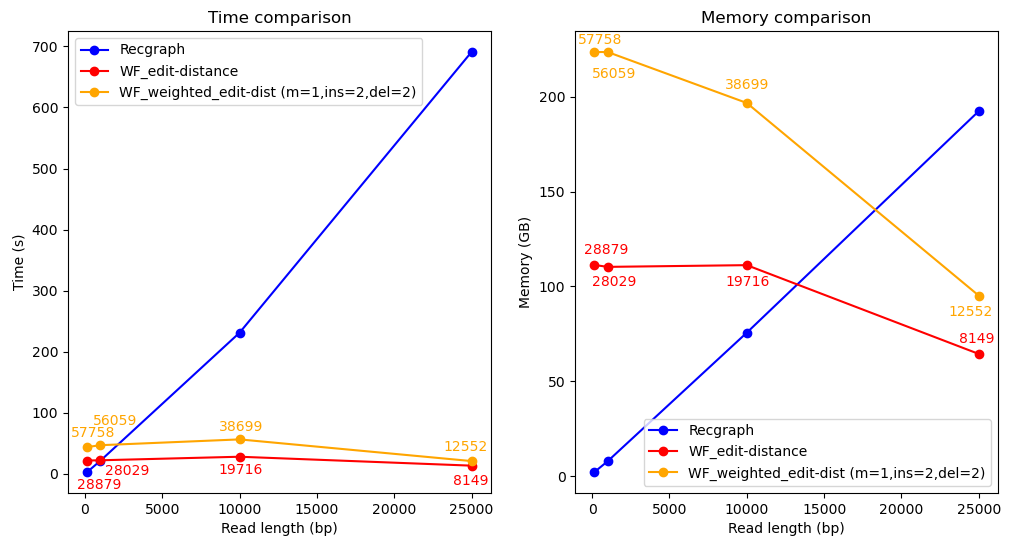
\includegraphics[width=1.0\linewidth]{images/global_comparison.png} 
        \caption[Confronto modalità globale]{Confronto in termini di tempo e spazio per l'allineamento in \textbf{modalità globale} tra \emph{RecGraph} e \emph{wf\_alignment\_edit-distance}. I numeri riportati rappresentano le \textbf{distanze di edit} computate da \emph{wf\_alignment\_edit-distance}.}
        \label{fig:global_comparison}
    \end{figure}
    \vspace{20pt}
    
    Nella \emph{modalità globale}, risulta poco sensato l'utilizzo di \textbf{\textit{wf\_edit-distance}} quando le sequenze sono molto \emph{più corte} dei cammini del grafo; al contrario, diventa estremamente interessante il suo impiego (sia in termini di \textbf{tempo di esecuzione} che di \textbf{memoria occupata}) quando la \emph{dimensione delle reads} diventa \emph{paragonabile} a quella dei \emph{cammini}, usando eventualmente anche \emph{penalità non unitarie}. 
    \clearpage
    
\subsubsection{Modalità semiglobale}
    Si riportano ora i risultati ottenuti ottenuti in \textbf{modalità semiglobale}, per la quale sono state usate \emph{reads} di lunghezza 150 bp, 1000 bp e 10000 bp; si mostrano per primi nuovamente i valori ottenuti utilizzando \textbf{\textit{RecGraph}}:
    \vspace{20pt}
    \begin{table}[h]
        \centering
        \begin{tabular}{|c|c|c|c|c|c|c|c|}
            \hline
                \multicolumn{8}{|c|}{\multirow{2}{*}{\textbf{Modality:} \emph{Semiglobal}}} \\
                \multicolumn{8}{|c|}{} \\
            \hline
                & \multicolumn{2}{|c|}{\textbf{Reads}} & \multicolumn{4}{|c|}{\textbf{Time (s)}} & \textbf{Memory (GB)} \\
            \hline
                \textbf{Algorithm} & \textbf{N} & \textbf{L} & \textbf{Tot} & \textbf{Mean} & \textbf{Max} &  \textbf{Min} & \textbf{Max} \\
            \hline
                \multirow{4}{*}{\emph{RecGraph}} & 100 & 150 & 270 & 2.7 & 3.1 & 2.3 & 2.67 \\
            \cline{2-8}
                & \multirow{2}{*}{25} & 1000 & \multirow{2}{*}{483} & 19.3 & 22.3 & 18.5 & 7.84 \\
                & & $6.7 \times$ & & $4.6 \times$ & $7.2 \times$ & $8 \times$ & $2.9 \times$ \\
            \cline{2-8}
                & \multirow{2}{*}{5} & 10000 & \multirow{2}{*}{1080} & 216 & 223 & 208.1 & 75.66 \\
                & & $66.7 \times$ & & $80 \times$ & $71.9 \times$ & $90.5 \times$ & $28.3 \times$ \\
            \hline
        \end{tabular}
        \caption{Benchmark per \emph{RecGraph} in \emph{modalità semiglobale}.}
        \label{tab:benchmark_RecGraph_semiglobal}
    \end{table}
    \vspace{20pt}
    
    Come da previsione, i risultati ottenuti sono molto simili a quelli della \textbf{modalità globale} (tabella \ref{tab:benchmark_RecGraph_global}): infatti, in entrambe le modalità, \textbf{\textit{RecGraph}} computa allo stesso modo l'intera \emph{matrice di programmazione dinamica}, mantenendo quindi la stessa \emph{complessità}: le differenze stanno nelle diverse \emph{condizioni iniziali} e nella selezione della \emph{soluzione ottimale}.
    
    Al contrario, i risultati ottenuti da \textbf{\textit{wf\_edit\_distance}} cambiano radicalmente:
    \vspace{20pt}
    \begin{table}[h]
        \centering
        \begin{tabular}{|c|c|c|c|c|c|c|c|c|}
            \hline
                \multicolumn{9}{|c|}{\multirow{2}{*}{\textbf{Modality:} \emph{Semiglobal}}} \\
                \multicolumn{9}{|c|}{} \\
            \hline
                & \multicolumn{2}{|c|}{\textbf{Reads}} & \multicolumn{4}{|c|}{\textbf{Time (s)}} & \textbf{Memory (GB)} & \textbf{Score} \\
            \hline
                \textbf{Algorithm} & \textbf{N} & \textbf{L} & \textbf{Tot} & \textbf{Mean} & \textbf{Max} & \textbf{Min} & \textbf{Max} & \textbf{Mean} \\
            \hline
                \multirow{4}{*}{\emph{wf\_edit-dist}} & 100 & 150 & 2.02 & 0.02 & 0.2 & 0.01 & 0.138 & $<5$ \\
            \cline{2-9}
                & \multirow{2}{*}{25} & 1000 & \multirow{2}{*}{2.869} & 0.1 & 0.3 & 0.1 & 0.212 & 22.5 \\
                & & $6.7 \times$ & & $5 \times$ & $1.5 \times$ & $10.0 \times$ & $1.34 \times$ & $1.5 \times$ \\
            \cline{2-9}
                & \multirow{2}{*}{5} & 10000 & \multirow{2}{*}{18.4} & 3.7 & 4.4 & 3.2 & 5.07 & 1051 \\
                & & $66.7 \times$ & & $185 \times$ & $22.0 \times$ & $320 \times$ & $36.7 \times$ & $260 \times$\\
            \hline
        \end{tabular}
        \caption{Benchmark per \emph{wf\_edit-distance} in \emph{modalità semiglobale}.}
        \label{tab:benchmark_wf_edit-dist_semiglobal}
    \end{table}
    \vspace{20pt}

    L'\textbf{allineamento semiglobale} permette di allineare le sequenze a qualsiasi punto del grafo, ottenendo \textbf{distanze di edit} nettamente inferiori che aumentano in maniera proporzionale alla lunghezza delle reads. Come conseguenza, anche \textbf{\textit{wf\_edit-distance}} scala in maniera proporzionale alla lunghezza delle sequenze. 

    \vspace{20pt}
    Di seguito un confronto dei valori ottenuti da \textbf{\textit{RecGraph}} e da \textbf{\textit{wf\_edit\_distance}} (sia con penalità unitarie che nel caso pesato) sulle sequenze di interesse:

    \begin{table}[h]
        \centering
        \begin{tabular}{|c|c|c|c|c|c|}
            \hline
             \multicolumn{2}{|c|}{\textbf{Modality:} \emph{Semiglobal}} & \multicolumn{2}{|c|}{\textbf{Reads number: } \emph{100}} & \multicolumn{2}{|c|}{\textbf{Reads length:} \emph{150 bp}} \\
            \hline
                \multicolumn{6}{|c|}{} \\
            \hline
                & \multicolumn{4}{|c|}{\textbf{Time (s)}} & \textbf{Memory (GB)} \\
            \hline
                \textbf{Algorithm} & \textbf{Tot} & \textbf{Mean} & \textbf{Max} & \textbf{Min} & \textbf{Max} \\
            \hline
                \emph{RecGraph} & 270 & 2.7 & 3.1 & 2.3 & 2.67 \\
            \hline
                \multirow{2}{*}{\emph{wf\_edit-distance}} & 2.02 & 0.02 & 0.2 & 0.01 & 0.138 \\
                & $<0.01 \times$ & $<0.01 \times$ & $0.06 \times$ & $<0.01 \times$ & $0.05 \times$ \\
            \hline
                \multirow{2}{*}{\emph{wf\_weighted\_ed}} & 3.27 & 0.024 & 0.2 & 0.01 & 0.165 \\
                & $0.01 \times$ & $0.01 \times$ & $0.06 \times$ & $<0.01 \times$ & $0.06 \times$ \\
            \hline
        \end{tabular}
        \caption{Benchmark per \emph{reads} di 150 bp in \emph{modalità semiglobale}. Nella modalità \textbf{\textit{wf\_weighted-edit-distance}}, sono state usate le seguenti penalità: \textbf{mismatch=1}, \textbf{insertion=2}, \textbf{deletion=2}.}
        \label{tab:benchmark_semiglobal_150}
    \end{table}
    \vspace{20pt}
    
    \begin{table}[h]
        \centering
        \begin{tabular}{|c|c|c|c|c|c|}
            \hline
                \multicolumn{2}{|c|}{\textbf{Modality:} \emph{Semiglobal}} & \multicolumn{2}{|c|}{\textbf{Reads number: } \emph{25}} & \multicolumn{2}{|c|}{\textbf{Reads length:} \emph{1000 bp}} \\
            \hline
                \multicolumn{6}{|c|}{} \\
            \hline
                & \multicolumn{4}{|c|}{\textbf{Time (s)}} & \textbf{Memory (GB)} \\
            \hline
                \textbf{Algorithm} & \textbf{Tot} & \textbf{Mean} & \textbf{Max} & \textbf{Min} & \textbf{Max} \\
            \hline
                \emph{RecGraph} & 483 & 19.3 & 22.3 & 18.5 & 7.84 \\
            \hline
                \multirow{2}{*}{\emph{wf\_edit-distance}} & 2.87 & 0.1 & 0.3 & 0.1 & 0.212 \\
                & $<0.01 \times$ & $<0.01 \times$ & $0.01 \times$ & $<0.01 \times$ & $0.03 \times$ \\
            \hline
                \multirow{2}{*}{\emph{wf\_weighted\_edit-distance}} & 3.22 & 0.1 & 0.4 & 0.1 & 0.351 \\
                & $<0.01 \times$ & $<0.01 \times$ & $0.02 \times$ & $<0.01 \times$ & $0.05 \times$ \\
            \hline
        \end{tabular}
        \caption{Benchmark per \emph{reads} di 1000 bp in \emph{modalità semiglobale}. Nella modalità \textbf{\textit{wf\_weighted-edit-distance}}, sono state usate le seguenti penalità: \textbf{mismatch=1}, \textbf{insertion=2}, \textbf{deletion=2}.}
        \label{tab:benchmark_semiglobal_1k}
    \end{table}
    \vspace{20pt}
    
    \begin{table}[h]
        \centering
        \begin{tabular}{|c|c|c|c|c|c|}
            \hline
                \multicolumn{2}{|c|}{\textbf{Modality:} \emph{Semiglobal}} & \multicolumn{2}{|c|}{\textbf{Reads number: } \emph{5}} & \multicolumn{2}{|c|}{\textbf{Reads length:} \emph{10000 bp}} \\
            \hline
                \multicolumn{6}{|c|}{} \\
            \hline
                & \multicolumn{4}{|c|}{\textbf{Time (s)}} & \textbf{Memory (GB)} \\
            \hline
                \textbf{Algorithm} & \textbf{Tot} & \textbf{Mean} & \textbf{Max} & \textbf{Min} & \textbf{Max} \\
            \hline
                \emph{RecGraph} & 1080 & 216 & 223 & 208.1 & 75.66 \\
            \hline
                \multirow{2}{*}{\emph{wf\_edit-distance}} & 18.4 & 3.7 & 4.4 & 3.2 & 5.07 \\
                & $0.02 \times$ & $0.02  \times$ & $0.02 \times$ & $0.02 \times$ & $0.08 \times$ \\
            \hline
                \multirow{2}{*}{\emph{wf\_weighted\_edit-distance}} & 18.8 & 3.8 & 4.3 & 3.4 & 5.68 \\
                & $0.02 \times$ & $0.02 \times$ & $0.02 \times$ & $0.02 \times$ & $0.08 \times$ \\
            \hline
        \end{tabular}
        \caption{Benchmark per \emph{reads} di 10000 bp in \emph{modalità semiglobale}. Nella modalità \textbf{\textit{wf\_weighted-edit-distance}}, sono state usate le seguenti penalità: \textbf{mismatch=1}, \textbf{insertion=2}, \textbf{deletion=2}.}
        \label{tab:benchmark_semiglobal_10k}
    \end{table}
    \vspace{20pt}
    
    e un \textbf{plotting} dei risultati appena riportati (figura \ref{fig:semiglobal_comparison}):
    \clearpage
    \begin{figure}[t]
        \centering
        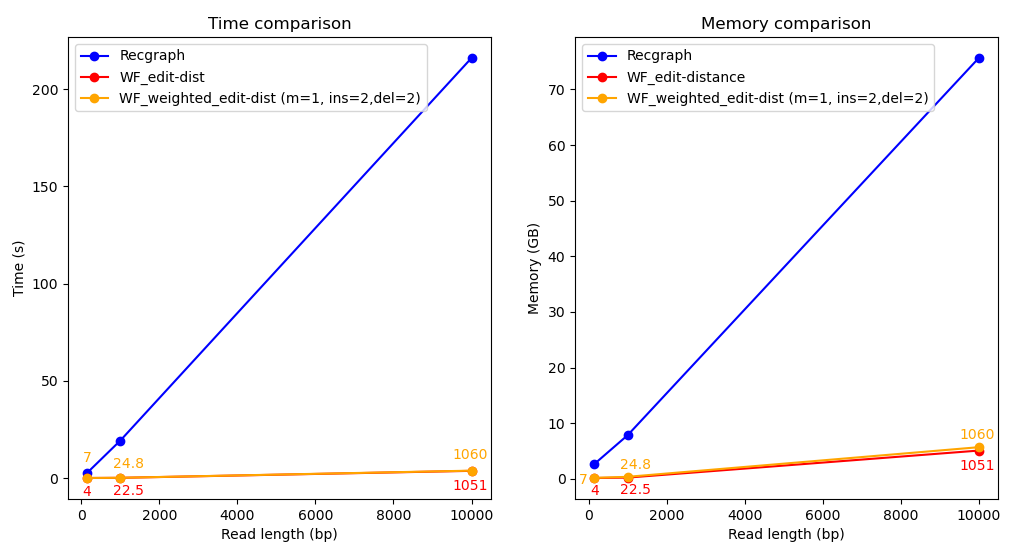
\includegraphics[width=1.0\linewidth]{images/semiglobal_comparison.png} 
        \caption[Confronto modalità semiglobale]{Confronto in termini di tempo e spazio per l'allineamento in \textbf{modalità semiglobale} tra \emph{RecGraph} e \emph{wf\_alignment\_edit-distance}. I numeri riportati rappresentano le \textbf{distanze di edit} computate da \emph{wf\_alignment\_edit-distance}.}
        \label{fig:semiglobal_comparison}
    \end{figure}
    
    Nella \textbf{modalità semiglobale}, \textbf{\textit{wf\_edit\_distance}} risulta superiore a \textbf{\textit{RecGraph}} su tutti gli input, sia in \textbf{tempo di esecuzione} che in \textbf{memoria}.
    
\subsection{Analisi dell'andamento del prototipo su singole variabili}

    In questa seconda parte del benchmark ci si è concentrati in maniera specifica sull'analisi dell'andamento asintotico di \textbf{\textit{wf\_edit\_distance}}: prese come riferimento $n$ variabili, si è andato a misurare l'andamento di ognuna di esse fissando la restanti $n-1$ come costanti. In particolare, si sono considerate le seguenti dimensioni:
    \begin{itemize}
        \item \emph{valore dell'allineamento};
        \item \emph{numero di threads} lanciati in parallelo;
        \item \emph{numero di cammini} del \emph{grafo di variazione}.
    \end{itemize}
    Si è utilizzato come input lo stesso grafo utilizzato in precedenza (tabella \ref{tab:graph}) e delle sequenze della stessa lunghezza dei suoi cammini, eseguendo allineamenti in \textbf{modalità globale}.
    
    Dove non specificato diversamente, il \textbf{cammino ottimale} è stato inserito a metà di tutti i percorsi; inoltre è stato utilizzato un \emph{singolo thread} (tranne ovviamente nella sperimentazione sul numero dei threads). Come implementazione del \emph{fronte d'onda} è stato scelto \textbf{\textit{wf\_vec}}. 
    
    Si ricorda che la \textbf{complessità temporale} attesa dell'algoritmo è
    \begin{equation}
        T(n, m, p, \overline{d}) = O(\min\{n, m\} \cdot \overline{d} \cdot p)
        \label{equation:wf_time_complexity_benchmark}
    \end{equation}
    mentre la \textbf{complessità in spazio} è
    \begin{equation}
        T(n, m, p, \overline{d}) = O((n+m) \cdot \overline{d} \cdot p)
        \label{equation:wf_space_complexity_benchmark}
    \end{equation}
    a causa dell'implementazione \textbf{\textit{wf\_vec}} scelta (equazione \ref{equation:space_complexity_wf_vec}).

    \vspace{20pt}
    A seguire i risultati ottenuti.

\subsubsection{Numero di threads variabile}
     \begin{figure}[h]
        \centering
        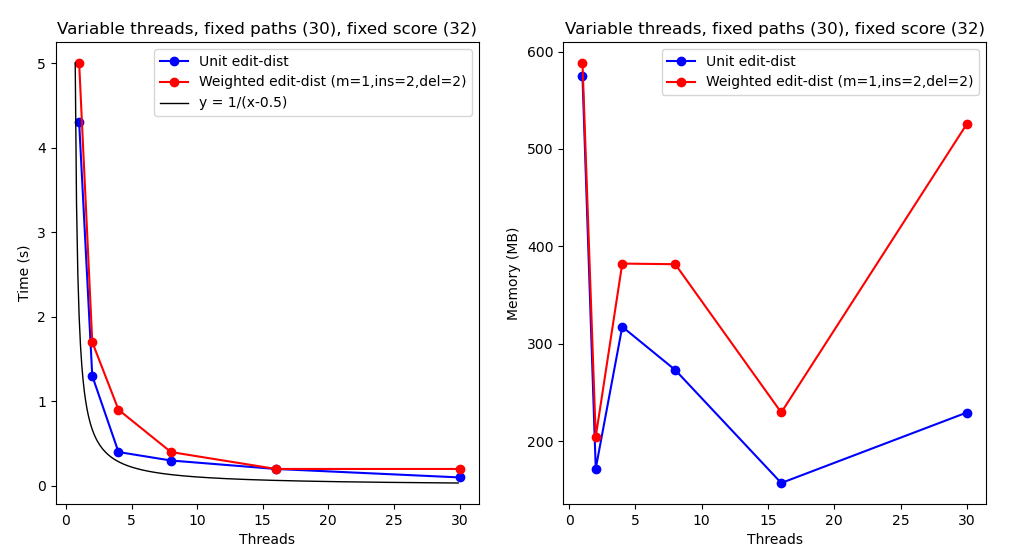
\includegraphics[width=1.0\linewidth]{images/benchmark_threads_variable.png} 
         \caption[Andamento con threads variabili]{Andamento in \emph{tempo} di \textbf{\textit{wf\_alignment}} rispetto a un \emph{numero di threads} eseguiti in parallelo \emph{variabile}.}
        \label{fig:benchmark_threads}
    \end{figure}
    \vspace{20pt}

    Facendo variare il \textbf{numero di threads} eseguiti in parallelo si evidenzia un \emph{andamento asintotico temporale} del tipo $y = \frac{1}{x}$, come da previsione. L'andamento in \emph{memoria} risulta molto più imprevedibile, anche in questo caso come conseguenza del troncamento rispetto all' allineamento migliore trovato, spiegato nella sezione \ref{section:wf_alignment}.
\clearpage

\subsubsection{Punteggio dell'allineamento variabile}
     \begin{figure}[h]
        \centering
        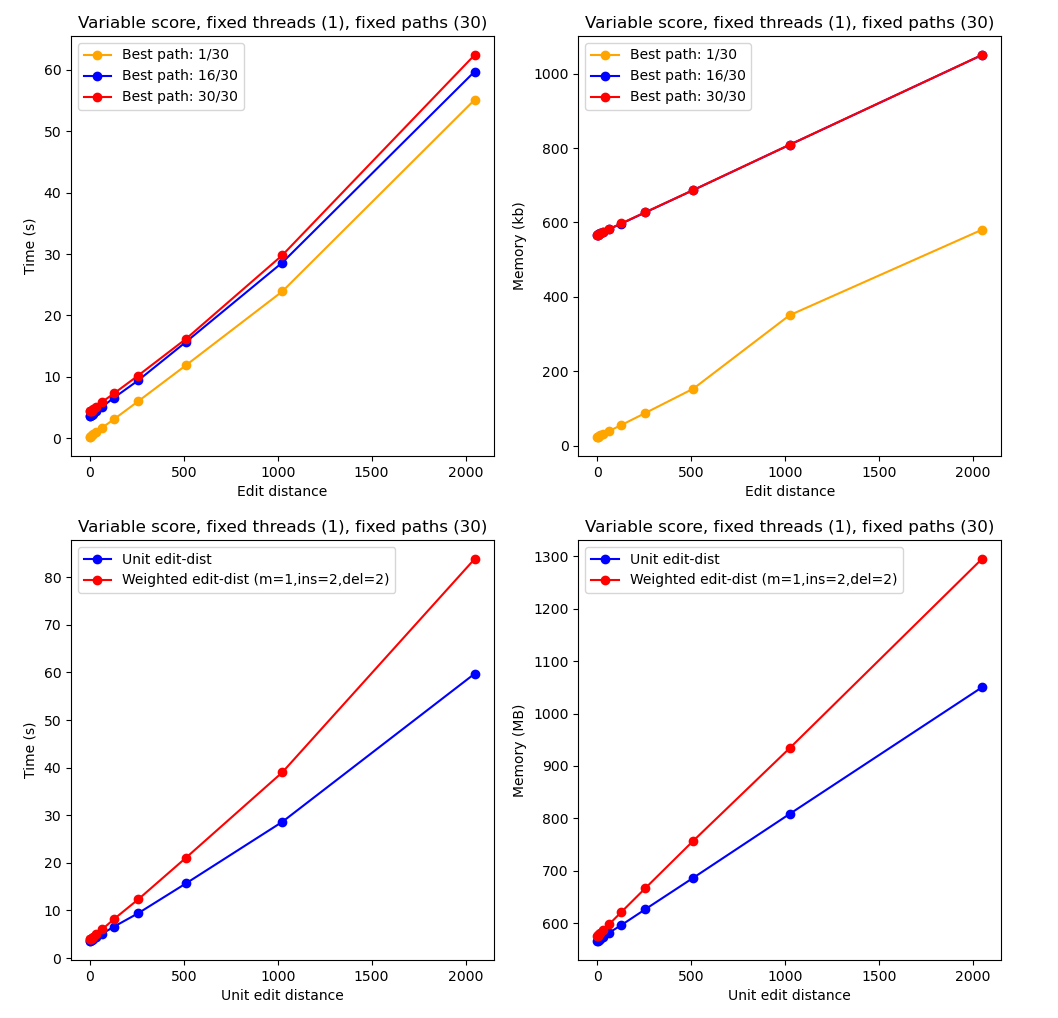
\includegraphics[width=1.0\linewidth]{images/benchmark_score_variable.png} 
        \caption[Andamento con score variabile]{Andamento in \emph{tempo} e in \emph{memoria} di \textbf{\textit{wf\_alignment}} rispetto a un \emph{punteggio} dell'allineamento \emph{variabile}.}
        \label{fig:benchmark_score}
    \end{figure}
    \vspace{20pt}
    
    Nella sperimentazione con \textbf{distanza di edit variabile} si nota un \emph{andamento lineare} sia in tempo che in memoria, in linea con le aspettative. Spostando la posizione del \emph{percorso ottimale} le rette mantengono lo stesso \textbf{coefficiente angolare}, variando nell'\textbf{ordinata all'origine} (conseguenza del troncamento rispetto alla soglia trovata, sezione \ref{section:wf_alignment}); aumentando le penalità, si nota un aumento dell'inclinazione della retta, conseguenza diretta della \emph{dipendenza lineare} nella \textbf{distanza di edit}.

\clearpage
\subsubsection{Numero di cammini del grafo variabile}
    \begin{figure}[h]
        \centering
        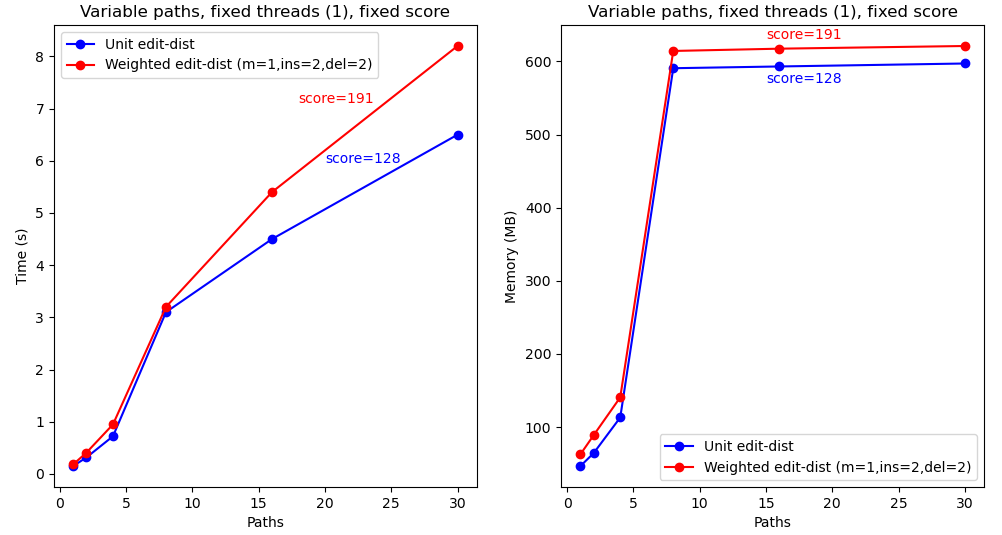
\includegraphics[width=1.0\linewidth]{images/benchmark_paths_variable.png} 
         \caption[Andamento con percorsi variabili]{Andamento in \emph{tempo} e in \emph{memoria} di \textbf{\textit{wf\_alignment}} rispetto a un \emph{numero di percorsi} del grafo \emph{variabili}.}
        \label{fig:benchmark_paths}
    \end{figure}
    \vspace{20pt}
    
    Nell'ultima sperimentazione, che considera il \textbf{numero di percorsi del grafo}, si ottengono risultati leggermente meno precisi dei precedenti, a causa dell'alta variabilità dell'input; infatti, il \emph{percorso ottimale} viene sempre inserito a metà dei percorsi disponibili: come conseguenza, i percorsi non ottimali (variabili) computati prima di quello ottimale provocano un andamento non completamente in linea con le equazioni \ref{equation:wf_time_complexity_benchmark} e \ref{equation:wf_space_complexity_benchmark}. Tuttavia, in assoluto è possibile comunque notare una \textbf{dipendenza lineare} nel \textbf{tempo di esecuzione}, mentre per quanto riguarda la \textbf{memoria} i risultati dipendono troppo dagli allineamenti trovati prima di quello ottimale.   

